\subsubsection{Security and performance measures used (D4)}
\label{security_performance}
Security and performance are two of the most important non-functional requirements for any software product. 
We asked three open-ended questions with regards to the enforcement of security and performance-related features in software products in Bangladesh:
How do you ensure security (Q23), performance (Q21), and scalability (Q22) in your software products?

% To identify general practices among the Bangladeshi software companies regarding software products' security and performance, we have included two open-ended questions in the survey. This particular question covers how a company secures its developed products from security threats and maintain performance after deployment. However, the scalability of software directly impacts its performance\citep{Liu2009,Bondi2000}. Hence, we will cover the following points here:
% \begin{itemize}
%     \item Security
%     \item Performance
%     \item Scalability
% \end{itemize}


%\label{Security}

\begin{figure}[h]
\centering
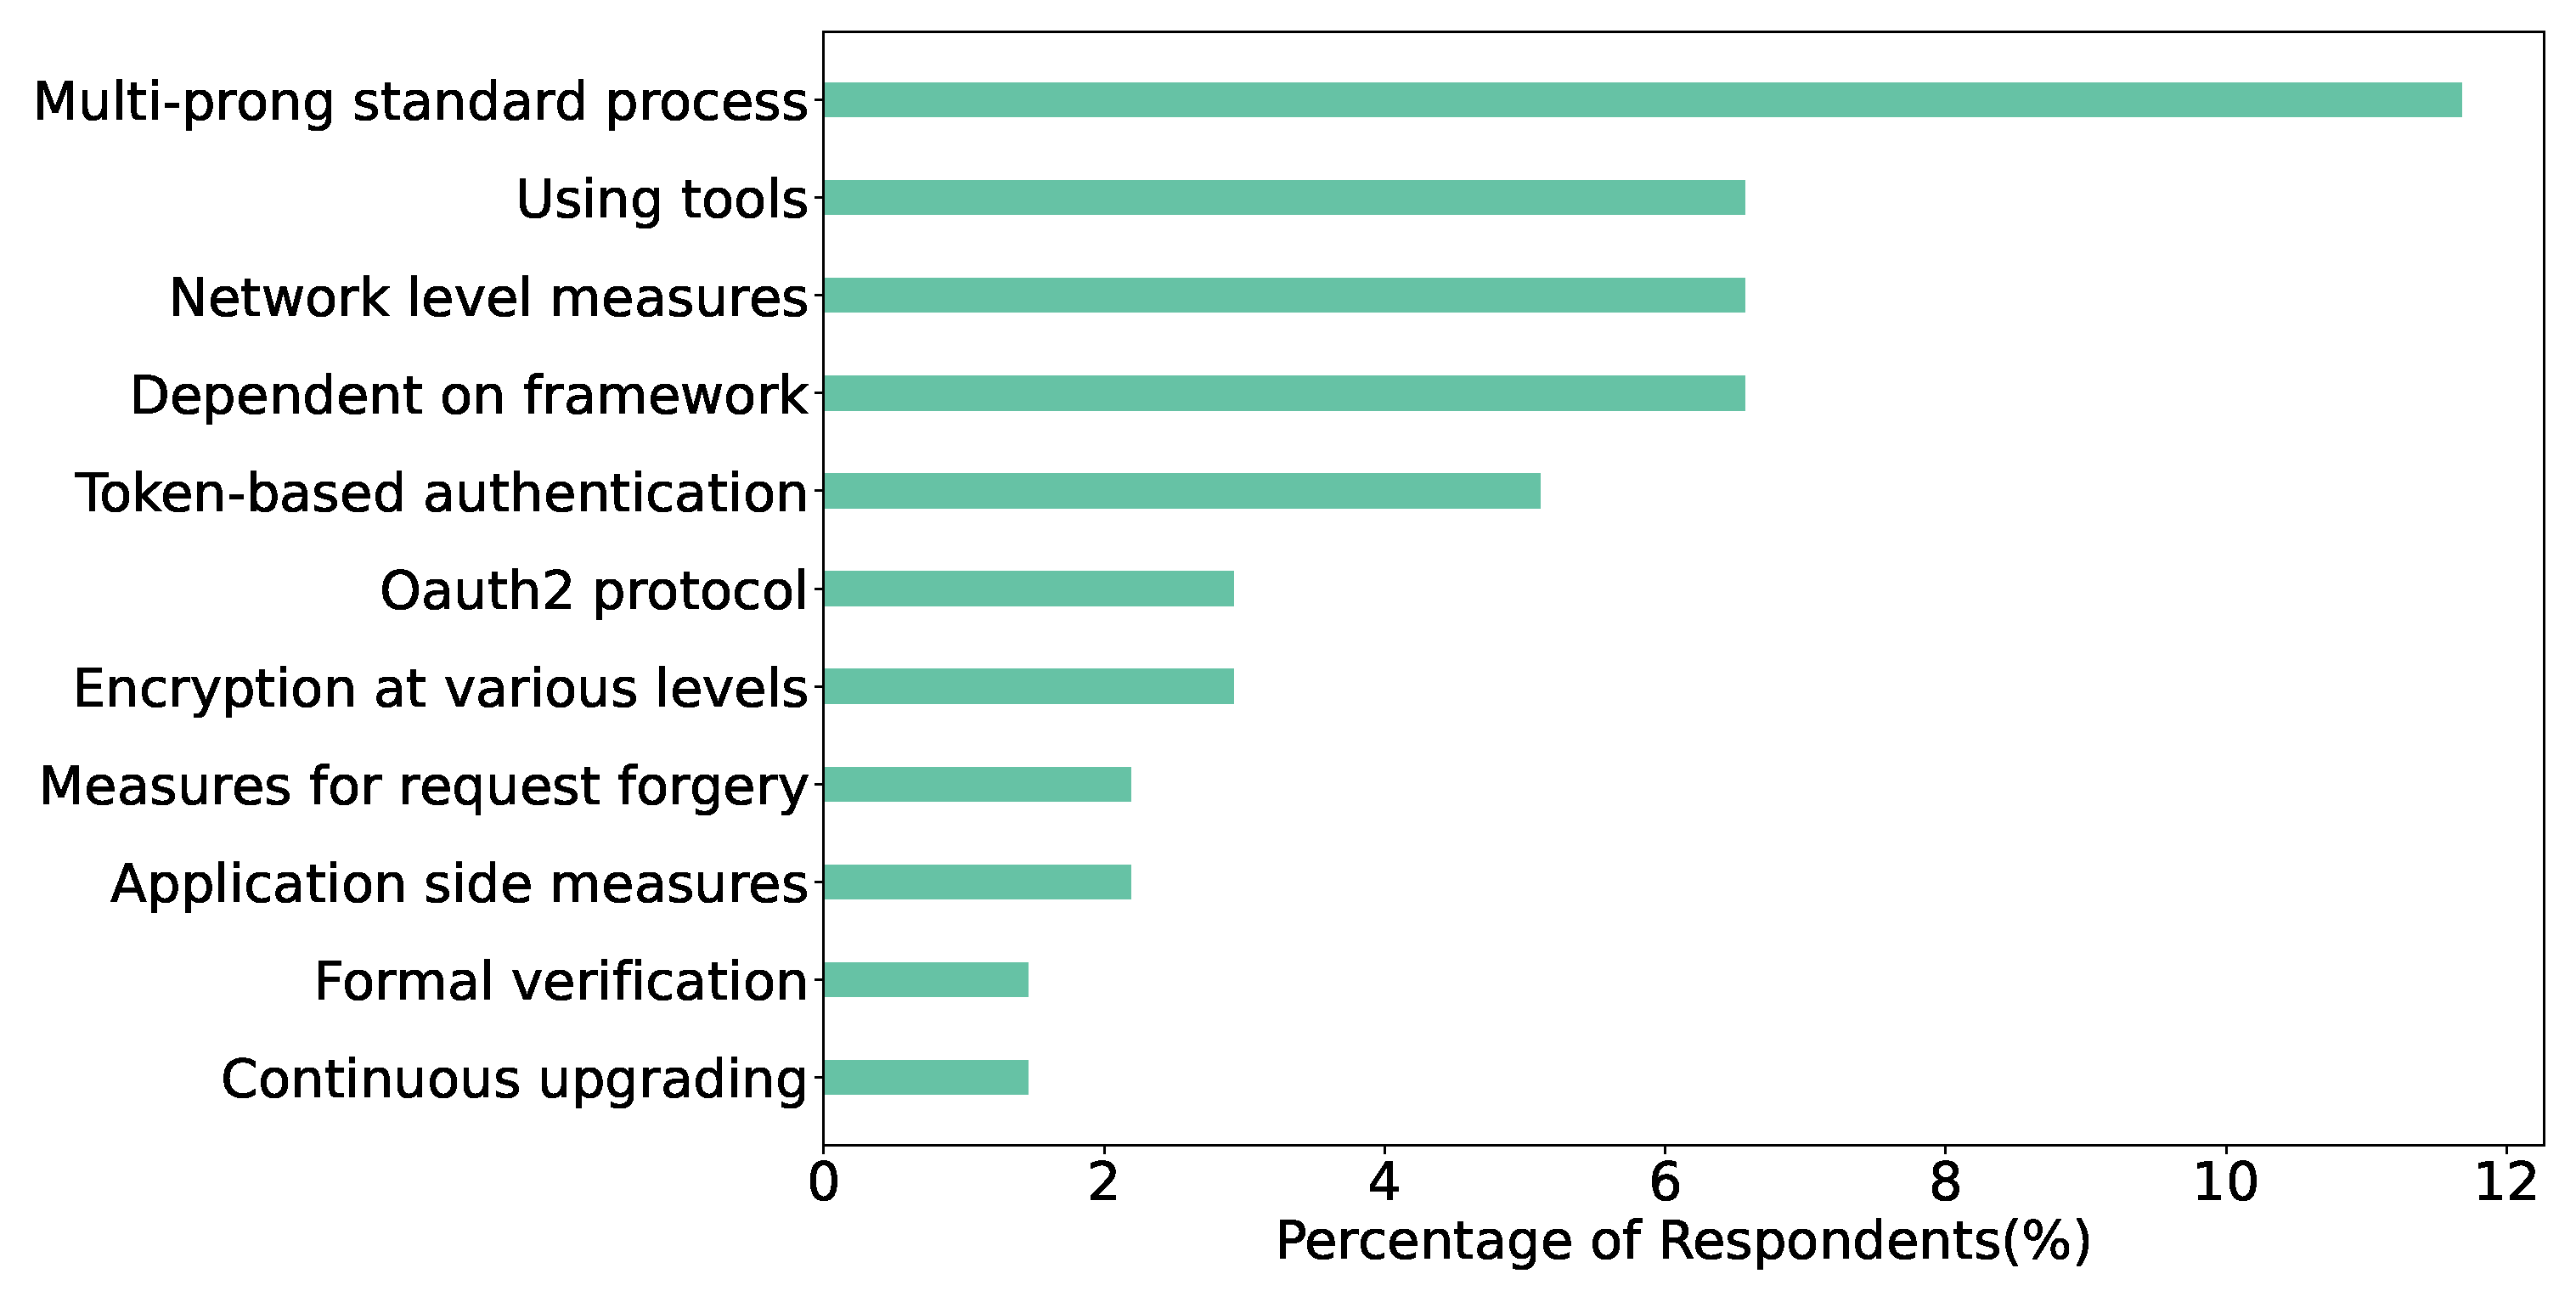
\includegraphics[scale=0.22]{Figures/Security.eps} 
\caption{Measures to ensure security of products}
\label{fig:Measures to ensure security}
\end{figure}
\nd\bf{$\bullet$ Security (Q23):} Our open coding of the survey responses reveals 11  
labels (see Figure \ref{fig:Measures to ensure security}). The 11 labels are are divided into three main categories of security-related development practices: 
\begin{inparaenum}
\item Measures related to authentication and authorization (64.82\%),
\item Exploitation of tools and techniques to ensure security in products (53.71\%), and 
\item Use of encryption technologies for data (7.41\%).
\end{inparaenum} We discuss the categories below.  


\begin{inparaenum}[(1)]
\item \ib{Measures related to authentication and authorization.} Six out of the 11 labels belong to this category. 
\begin{inparaenum}
\item \it{Multi-prong Standard Process}. About 29.6\% of the respondents
reported that they practice various security standards and protocol to
ensure security (e.g., ISO/IEC 27001, PA DSS).
\item \it{Token-based authentication.} About 13\% respondents reported to 
have implemented a token-based authentication system, which 
allows users to enter their username and password to obtain a token for authentication and authorization.
\item \it{OAuth 2.0} : Around 7.4\%) respondents use the OAuth 2.0
protocol as the primary way of maintaining security. OAuth 2.0 is the industry-standard protocol for
authorization. OAuth 2.0 focuses on client developer simplicity while providing
specific authorization flows for web applications, desktop applications, mobile
phones, and living room devices. %, e.g., \emt{OAuth 2.0,
\item \it{Application-side measures}: Around 5.6\% of respondents 
implement security measures at the application level like encryption of application data at the client-side, use of https while
pulling data from a server, secured architecture, etc.
\item \it{Measures for request forgery}: Around 5.6\% respondents implemented security measures against
Cross-site request forgery (e.g., attacks like
cross-origin resource sharing (CORS), cross-site request forgery (CSRF) or
one-click attack or XSRF). Security testing is paramount for this: \emt{Security testings
like: SQL injection, cross-site scripting, CSRF, API security, use of https, 
detecting malicious/suspicious HTTP requests and auto-blocking} (Respondent ID $S_{42}$)
    \item \it{Formal Verification}: Around 3.7\% respondents ensured the practice of formal code review to enforce security practices: \emt{There are some basic
    guidelines that we must follow and while code review this needs to be an
    absolute part that needs to be checked before the code gets merged} ($S_{112}$)
    \end{inparaenum}

\item \ib{Exploitation of tools and techniques to ensure security in products.} Four out of the 11 labels belong to this category. 
\begin{inparaenum}
  \item \it{Dependent on Framework}: Around 16.7\% 
  respondents depend on the underlying framework for security like Spring, HDIV, and Laravel. 
  \emt{https, popular framework which already prevents some type of attacks. rest of the things on case-by-case basis)}($S_{79}$)
  \item \it{Use of tools}: Respondents use various open-source/paid tools for
  scanning and testing like OWASP and penetration testing tools.
  %\emt{use encryption at different level of software (server, network, transmission layer, database and software layer.)}{35}
  \item \it{Network level Measures}: Network-level measures include
  IP-white-listing, port-blocking, VPN, and the use of HTTPS in software.
  16.7\% of respondents use at least one of the mentioned strategies to ensure
  security.
  %\emt{network blocking and common security measures}{2}
  \item \it{Continuous Upgrade}: Around 1.5\% 
  respondents reported that they arrange frequent hackathons, workshops, and
  security audits: \emt{We run security audit of our office environment. We also conduct security session per 6 months to introduce latest trend in threats and what we can do to avoid it}($S_{57}$)
\end{inparaenum}

\item \ib{Use of encryption technologies for data}. Around 7.4\% respondents use encryption at
the different levels of software architecture such as network, data, and
transmission.
\emt{use encryption at different level of software (server, network, transmission layer, database and software layer.)}($S_{35}$)
\end{inparaenum}
% 
% Authentication and authorization based security are the most prominent practices in the software industry of Bangladesh. The other techniques used widely include framework, platform, tools, and encryption. Under these categories, several measures are usually followed. The security measures of the Bangladesh SE industry is presented in Figure \ref{fig:Measures to ensure security}. The measures of each category are discussed below.
% 
% Measures under the \emph{authentication and authorization} category is practised by 53.71\% respondents to ensure security. The measures are 
% \begin{enumerate}[label=(\alph*)]
% 
%     \item \textbf{Multi-prong Standard Process}: About 29.63\% of the respondents reported that they practice various security standards and protocol to ensure security. The standard includes ISO/IEC 27001 and PA DSS.
%     \surveyquote{Multi Prong Standard Processes and Products}{110}
%     
%     \item \textbf{Token-based authentication}: A token-based authentication system allows users to enter their username and password to obtain a token, which allows them to fetch a specific resource without using their username and password. Once their token has been obtained, the user can offer the token, which offers access to a specific resource for a time period to the remote site. 12.96\% of people expressed its eligibility.
%     \surveyquote{Token based authentication for all of my rest service}{80}
%     
%     \item \textbf{OAuth 2.0} : OAuth 2.0 is the industry-standard protocol for authorization. OAuth 2.0 focuses on client developer simplicity while providing specific authorization flows for web applications, desktop applications, mobile phones, and living room devices. Many (7.41\%) respondents use the OAuth 2.0 protocol as the primary way of maintaining security.
%     \surveyquote{OAuth 2.0, JWT, Token Based Authentication, CORS Filter, XSRF}{127}
%     
%     \item \textbf{Application-side measures}: 5.56\% of respondents responded that they would implement security measures at the application level. This measure includes encryption of application data at the client-side, use of https while pulling data from a server, secured architecture, etc.
%     \surveyquote{At application level, could not achieve others yet}{72}
%     
%     \item \textbf{Measures for request forgery}: Cross-site forgery attacks include cross-origin resource sharing (CORS), cross-site request forgery (CSRF) or one-click attack or XSRF. 5.56\% of respondents implemented measures against  Cross-site request forgery to ensure security.
%     \surveyquote{Security testings like: SQL injection, cross-site scripting, CSRF, API security, use of https,  detecting malicious/suspicious HTTP requests and auto-blocking}{42}
%     
%     \item \textbf{Formal Verification}: A code-level review can mitigate security threats. 3.7\% respondents ensured the practice of formal code review.
%     \surveyquote{There are some basic guidelines that we must follow and while code review this needs to be an absolute part that needs to be checked before the code gets merged}{112}
%     
% \end{enumerate}

% 53.71\% respondents exploit several technologies, tools, and platforms to ensure the security of their products. Measures under the \emph{framework/platform/tools} can be categorized as follows:
% 
% \begin{enumerate}[label=(\alph*)]
%   \item \textbf{Dependent on Framework}: The common frameworks provide basic to intermediate level security measures in the application. 16.67\% of respondents depend on the framework for security. The frameworks include popular ones such as Spring and HDIV. We have found that respondents using Spring and Laravel framework mostly reported depending on the framework for security. However, the observation is not statistically significant.
%   \surveyquote{https, popular framework which already prevents some type of attacks. rest of the things on case-by-case basis)}{79}
%   
%   \item \textbf{Use of tools}: Respondents use various open-source/paid tools for scanning and testing. These tools help to find security threats in an existing system. The tools include OWASP provided and penetration testing tools.
%   \surveyquote{use encryption at different level of software (server, network, transmission layer, database and software layer.)}{35}
%   
%   \item \textbf{Network level Measures}: Network-level measures include IP-white-listing, port-blocking, VPN, and the use of HTTPS in software. 16.67\% of respondents use at least one of the mentioned strategies to ensure security.
%   \surveyquote{network blocking and common security measures}{2}
% 
%   \item \textbf{Continuous Upgrade}: As security threats evolve continuously, the applications need continuous up-gradation at a frequent interval. 1.46\% of respondents said that they would arrange frequent hackathons, workshops, and security audits to address the continuously evolving security threats.
%   \surveyquote{We run security audit of our office environment. We also conduct security session per 6 months to introduce latest trend in threats and what we can do to avoid it}{57}
% \end{enumerate}

%\boxtext{Security testing and the use of security standards are prevalent in the Bangladesh SE industry.}


% To maintain security of software product SE industry of Bangladesh is mainly dependent on standard process which includes cloud based security, third party software, OS hardening followed by uses of security tools, network level measures and framework security. As found by Harrison et al.\citep{Harrison2010} network level measures are the first choice in ensuring security of software product which matches with our findings. Srinivasan et al.\citep{Srinivasan2017} listed top 10 web framework in terms of security testing where Spring framework achieved 7\textsuperscript{th} position. From figure ~\ref{fig:frameworks} we have seen that most of our respondents use Spring framework for software development. This might be the reason that a lot number of respondents dependent on framework for ensuring security.


\begin{figure}[h]
\centering
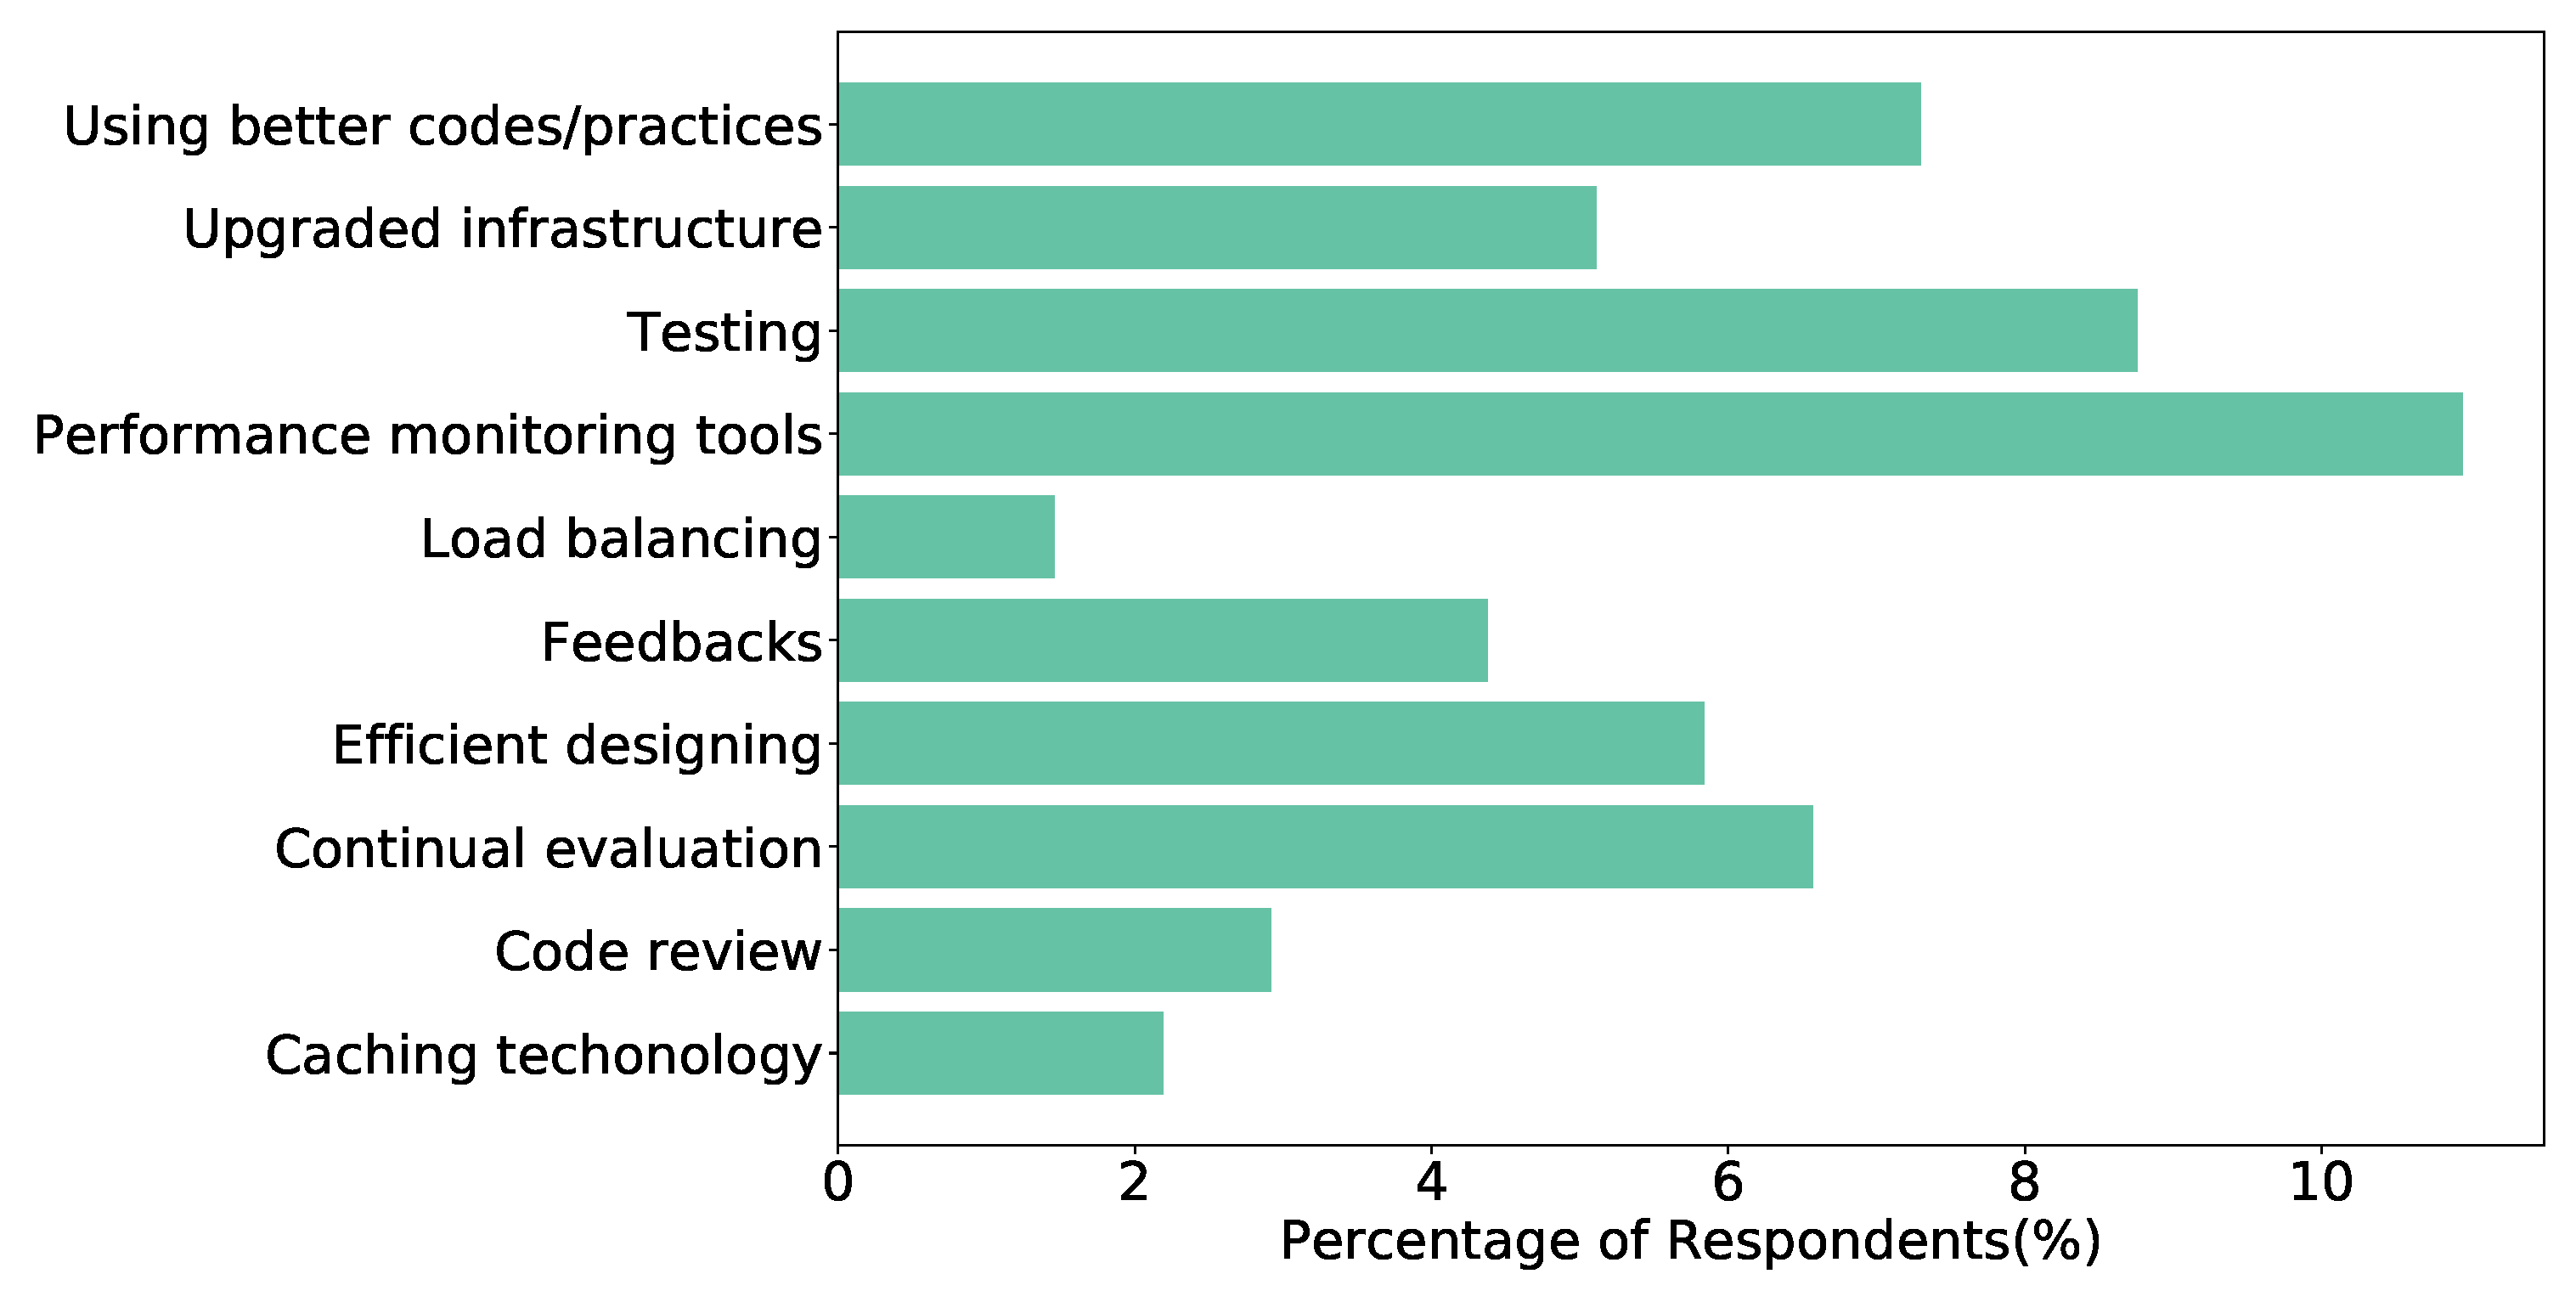
\includegraphics[scale=0.22]{Figures/Performance.eps} 
\caption{Measures to ensure performance of products}
\label{fig:Measures to ensure performance}
\end{figure}
\nd\bf{$\bullet$ Performance (Q21, Q22).} Software performance indicates how efficient the software is in terms of response time and resource consumption. 
We find nine types of performance measures that are practised in software products developed in Bangladesh (see Figure \ref{fig:Measures to ensure performance}).  
The nine types are divided into four categories: 
\begin{inparaenum}
Use of \item tools and frameworks (58.2\%),
\item design principles/best practices (32.7\%),
\item testing (21.8\%), and
\item review and feedback (21.8\%).
\end{inparaenum} 

\begin{inparaenum}[(1)]
\item \ib{Exploitation of tools and frameworks.} Four out of nine types belong to this category.
\begin{inparaenum}%[label=(\alph*)]
    \item \it{Tools}: Around 36.4\% respondents use tools and metrics to
    measure performance:  \emt{take help of different performance monitoring tools and dashboard, analyzed data, measure time and memory efficiency of process}($S_{35}$)
    \item \it{Infrastructure}: Around 12.7\% of respondents use upgraded
    infrastructure to ensure performance like cloud
    hosting (e.g., Amazon AWS), a high-end server, and new technologies.
    %\emt{Amazon Hosting and Quality Software}{85}
    \item \it{Caching}: Around 5.5\% respondents implemented caching to maintain
    software performance.
    % \emt{... Good Caching}{29}
    \item \it{Load Balancing}: Around 3.6\% respondents use load
    balancing as a measure to maintain performance:
    \emt{Optimizing number of HTTP requests, Asynchronous programming, Caching, CDN, Load Balancing, nginx, varnish, compression of data, 
    Continuous monitoring, Load testing, stress testing}($S_{42}$)
\end{inparaenum}
 
\item \ib{Use of design principles/best practices.}  Around 32.7\% respondents try to ensure software performance right from the design phase as follows.
\begin{inparaenum}%[label=(\alph*)]
    \item \it{Using better codes/practices}: Around 18.2\% respondents ensure performance by
    implementing industry-standard best practices like compression
    technology, enforcing design patterns, and refactoring.
    %\emt{Implementation time carefulness and maintaining a well developed coding standard}{40}
    \item \it{Efficient designing}: Around 14.6\% of respondents emphasize on
    performance-aware architecture design.
    %\emt{By careful designing}{24}
\end{inparaenum}

\item \ib{Use of testing.} Around 21.8\% respondents rely on the software testing strategy to ensure performance like load testing and stress testing.

\item \ib{Use of review and feedback.} Around 18.2\% of our respondents use user feedback (e.g., continuous feedback from QA team $S_{65}$) 
and code review to improve product performance. According to $S_{15}$: \emt{The code quality is assessed by the different team members during code review, followed by designing new ways to solve issues in the product that are time-intensive.}
\end{inparaenum}
% 
% Software performance indicates how efficient the software is in terms of response time and resource consumption. Our open coding of the survey responses reveals four main categories of performance-related development practices: 
% The measures are presented in Figure \ref{fig:Measures to ensure performance}.

% 
%  The use of framework/tools/platform to ensure software performance is a dominant (58.18\%) practice in the SE industry. Respondents in our survey reported multiple measures under these categories.
%  The measures belonging to \emph{framework/tools/platform} category are as follows:
% 
% \begin{enumerate}[label=(\alph*)]
%     \item \textbf{Performance Monitoring Tools}: There are various automated performance monitoring tools from which we can measure the overall and component-wise performance. 36.36\% of respondents use these tools to measure performance. Respondents use several performance metrics such as error/crash rate, response time, uptime, etc.
%     \surveyquote{take help of different performance monitoring tools and dashboard, analyzed data, measure time and memory efficiency of process}{35}
%     
%     \item \textbf{Upgraded Infrastructure}: 12.73\% of respondents use upgraded infrastructure to ensure performance. This infrastructure includes cloud hosting, a high-end server, and new technologies.
%     \surveyquote{Amazon Hosting and Quality Software}{85}
%     
%     \item \textbf{Caching Technology}: Caching mechanism improves performance by reducing response time. 5.45\% of respondents rely on caching to maintain software performance.
%     \surveyquote{... Good Caching}{29}
%     
%     \item \textbf{Load Balancing}: Load balancing can improve the system performance by ensuring an equal load to all servers. 3.64\% of respondents use load balancing as a measure to maintain performance.
%     \surveyquote{Optimizing number of HTTP requests, Asynchronous programming, Caching, CDN, Load Balancing, nginx, varnish, compression of data, Continuous monitoring, Load testing, stress testing}{42}
% 
% \end{enumerate}
% 
% 
% 32.73\% of respondents try to ensure software performance right from the design phase. Measures of this category are as follows:
% 
% \begin{enumerate}[label=(\alph*)]
% 
%     \item \textbf{Using better codes/practices}: Industry-standard best practices can improve system performance. 18.18\% respondents ensure performance by implementing best practices. The best practices include compression technology, enforcing design patterns, and refactoring.
%     \surveyquote{Implementation time carefulness and maintaining a well developed coding standard}{40}
%     
%     \item \textbf{Efficient designing}: Software performance is dependent on the architecture of the system. 14.55\% of respondents emphasize on performance-aware design to ensure performance.
%     \surveyquote{By careful designing}{24}
% 
% \end{enumerate}
% 
% 21.82\% of respondents of our survey relies on the software testing strategy to ensure performance. Performance testing includes load testing and stress testing.\anindya{Integration testing is not performance testing.}\partha{updated}
%  \surveyquote{By rigorous testing and checking performance testing}{17}
%  
%  Peer code review, user and tester feedback can be a good strategy to ensure performance. 18.18\% of our respondents use measures from this category to ensure performance. Measures under this category are:
%  
%  \begin{enumerate}[label=(\alph*)]
%  
%      \item \textbf{User Feedback}: It is a great source of performance measure. Taking time to time feedback from the clients helps a company realize how their products are performing. Many (10.91\%) respondents have highly recommended it.
%     \surveyquote{Continuous feedback from clients and QA team}{65}
%     
%     \item \textbf{Code Review}: About 7.27\% people have said that a proper and attentive code review can reduce the codes' faults and, therefore, enhance the performance of a software.
%     \surveyquote{The code quality is assessed by the different team members during code review, followed by designing new ways to solve issues in the product that are time-intensive.}{15}
%  
%  \end{enumerate}
%\boxtext{For performance, the SE industry in Bangladesh is largely dependent on monitoring tools and software testing.}


\paragraph{Scalability}
\label{Scalability}
\begin{figure}[h]
\centering
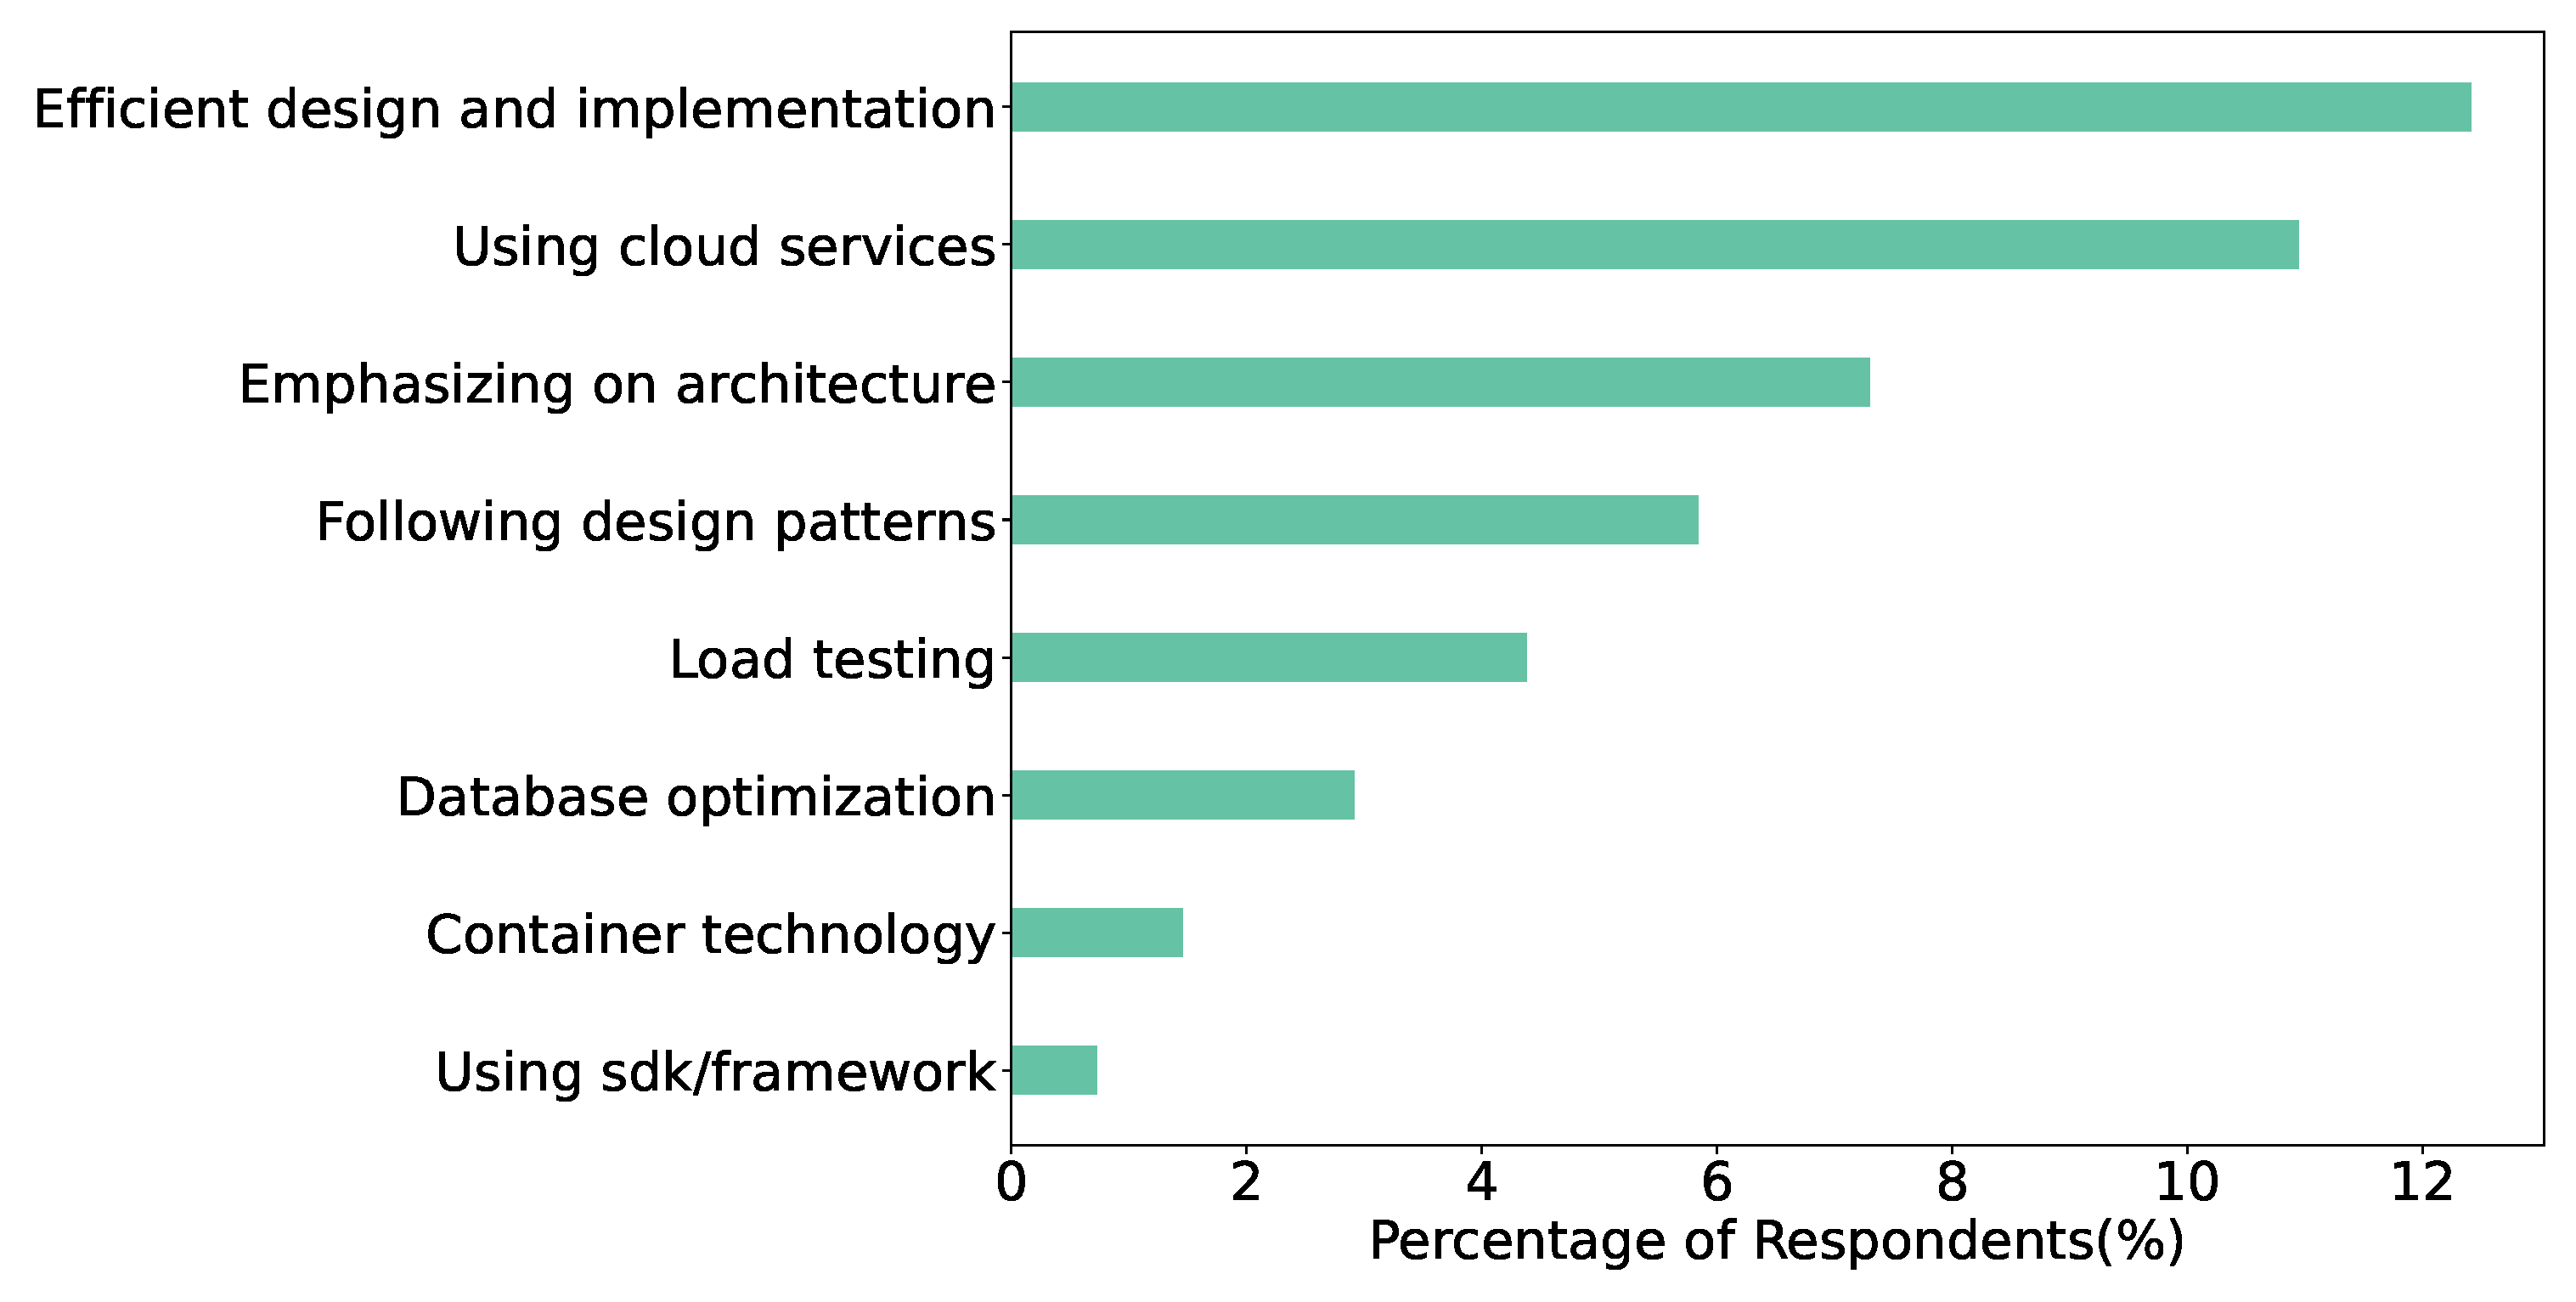
\includegraphics[scale=0.22]{Figures/Scalability.eps} 
\caption{Measures to ensure scalability of products}
\label{fig:Measures to ensure scalability}
\end{figure}

 Software scalability defines the ability to scale up a solution. Issues with little importance can impede scaling up. Thus proper measures should be taken from the design stage to ensure the scalability of the system. Scalability ensured by efficient software design is the most common strategy in the Bangladesh SE industry. Our open coding of the survey responses reveals four main categories of scalability-related development practices: 
\begin{inparaenum}
\item Use of design principles to ensure software scalability (67.3\%).
\item Exploitation of tools and frameworks to ensure software scalability (34.62\%). 
\item Use of testing to ensure software scalability(11.54\%), and
\item Use of database design standards to ensure software scalability (7.69\%).
\end{inparaenum} 
The measures practiced in the Bangladesh SE industry are presented in Figure \ref{fig:Measures to ensure scalability}.


 Scalability ensured by efficient software design is the most common strategy in the Bangladesh SE industry. 67.3\% reported using at least one of the measures in this category. The measures in \emph{efficient software design} category are:
% Recent days the cloud services offer tools to accomodate custom reactive scaling strategies. Thus, it has become easier to ensure scalability using cloud services \citep{Falatah2014}. Our results  also follows the world trend, usage of cloud services has placed 2\textsuperscript{nd} in terms popularity of scalability measures in SE industry of Bangladesh.
 \begin{enumerate}[label=(\alph*)]
 
     \item \textbf{Efficient Design and Implementation}: 32.69\% of respondents emphasize on the design and implementation of a scalable architecture. 
    \surveyquote{During implementation we always keep in mind about the scaling factor}{40}
    
     \item \textbf{Emphasizing on architecture}: 19.23\% of respondents emphasized on architecture. It is mostly micro-service architecture which they use to ensure scalability.
    \surveyquote{We follow the micro-service architecture. In a nutshell, we scale up the module vertically which is necessary. We use docker along with Jenkins for automatic deployments and scaling.}{10}

    
    \item \textbf{Following Design Patterns}: Some design patterns inherently help in scaling. 15.38\% of respondents think that implementing these design patterns will be of great use for software scalability.
    \surveyquote{Following certain design patterns}{8}
 
 \end{enumerate}
 
34.62\% of respondents of our survey use framework or tool to ensure scalability. The measures in this category are as follows:
\begin{enumerate}[label=(\alph*)]

    \item \textbf{Using Cloud Services}: 28.85\% users depend on cloud services such as AWS and Azure for the scalability of the system. Modern features like elastic load balancing and auto-scaling make it easy to ensure scalability.
    \surveyquote{Using AWS Elastic Load Balancer}{28}
    
    \item \textbf{Container Technology}: Container technologies include Docker, Kubernetes, etc. which ensure OS-level virtualization. By standardizing the system, container technologies ease the scaling of infrastructure. 3.85\% of the respondents use these measures to ensure product scalability. Containers enable users to scale their system without any dependency on the underlying OS.
    \surveyquote{We used Docker technology}{85}
    
    \item \textbf{Using SDK/framework}: Modern frameworks ensure scalability by default. 1.92\% of respondents solely depend on the framework for scalability.
    \surveyquote{following flexible framework which allows better scalability}{14}
  
\end{enumerate}
 
 
There is one measure under the software testing category, which is load testing. Load testing can be used to check the scalability of a system. 11.54\% of respondents use load tests to check whether their system is scalable or not.
\surveyquote{through load testing and load simulation.}{35}

There is also one measure under the Database Design category, which is database optimization. Database optimization includes sharding, clustering, indexing, and scaling. 7.69\% of respondents optimize the database to scale their system.
\surveyquote{Besides scaling horizontally, database scaling is performed by partitioning tables, along with multi-threaded implementations}{85}
%\boxtext{Typically software scalability is considered at the design phase in the SE industry of Bangladesh.}
%\boxtext{The use of cloud services is one of the common measures to ensure scalability.}
\begin{tcolorbox}[flushleft upper,boxrule=1pt,arc=0pt,left=0pt,right=0pt,top=0pt,bottom=0pt,colback=white,after=\ignorespacesafterend\par\noindent]
\nd\it{\bf{RQ1-D4. Security and performance measures used.}} Bangladesh software
industry uses various methods to ensure security, but the adoption of tools is not widespread. 
We have noticed that the Bangladesh
software industry mostly uses performance monitoring tools and software testing
to ensure product performance. Software scalability is generally considered at
the design stage (e.g., efficient design) in the Bangladesh SE industry. 
\end{tcolorbox}